% Shared preamble and frames for the three 5-minute talks.
% Each talk sets \presenter{...} before % Shared preamble and frames for the three 5-minute talks.
% Each talk sets \presenter{...} before % Shared preamble and frames for the three 5-minute talks.
% Each talk sets \presenter{...} before % Shared preamble and frames for the three 5-minute talks.
% Each talk sets \presenter{...} before \input{common}.
\usepackage{amsmath,amssymb}
\usepackage{booktabs}
\usepackage{xcolor}
\usetheme{MBZUAI}
\graphicspath{{assets/}{../figs/}}
\setbeamertemplate{navigation symbols}{}

\newcommand{\lam}{\lambda}
\newcommand{\strong}[1]{\textcolor{mbzuai-navy}{\textbf{#1}}}
\newcommand{\good}[1]{\textcolor{green!45!black}{\textbf{#1}}}
\newcommand{\bad}[1]{\textcolor{red!65!black}{\textbf{#1}}}

% ── Team and roles: edit here, all three decks update ─────────────────────
\newcommand{\roleJH}{Problem and setup; score cache and data pipeline; Q1 analysis; overall study (Q1--Q4)}
\newcommand{\roleLJ}{Continual learning experiments and analysis (Q2--Q3)}
\newcommand{\roleMA}{Downstream question-answering evaluation (Q4)}

\title[Fusion Weight for Keyframe Search]{Should the Fusion Weight Change with the Question?}
\institute[MBZUAI]{CV805 Course Project \\ Mohamed bin Zayed University of Artificial Intelligence}
\date{\today}
\titlelogos{assets/logo_dark.pdf}
\footleft{Should the Fusion Weight Change with the Question?}
\footright{\insertframenumber{} / \inserttotalframenumber}

% Team slide; #1 = JH, LJ or MA, the presenter's row is highlighted.
\usepackage{etoolbox}
\newcommand{\teamrow}[4]{% #1 key, #2 presenter key, #3 name, #4 role
  \ifstrequal{#1}{#2}%
    {\textbf{\textcolor{mbzuai-navy}{#3}} & \textbf{\textcolor{mbzuai-navy}{#4}} & \textcolor{mbzuai-dark-sand}{\textbf{this talk}}}%
    {\textcolor{mbzuai-subtle}{#3} & \textcolor{mbzuai-subtle}{#4} & }}
\newcommand{\teamframe}[1]{%
\begin{frame}{Team and my part}
  \centering
  \renewcommand{\arraystretch}{1.6}
  \begin{tabular}{p{0.27\textwidth}p{0.52\textwidth}p{0.11\textwidth}}
    \toprule
    Member & Main contribution & \\
    \midrule
    \teamrow{JH}{#1}{Jianxiang He}{\roleJH} \\
    \teamrow{LJ}{#1}{Longtao Jiang}{\roleLJ} \\
    \teamrow{MA}{#1}{Makhmud Assentay}{\roleMA} \\
    \bottomrule
  \end{tabular}
\end{frame}}

% Context frame used by every talk: VSI, the weight, and the example.
\newcommand{\contextframe}{%
\begin{frame}{Background: two clues, one weight}
  \begin{columns}[c,onlytextwidth]
    \begin{column}{0.47\textwidth}
      \small
      A VLM can only look at \strong{about 8 frames} of a long video, so we must pick them well.\\[2mm]
      VSI scores every second with two clues:
      \begin{itemize}
        \item \strong{Visual}: do the question's objects appear?
        \item \strong{Subtitle}: does the subtitle match the question?
      \end{itemize}
      \[ S(t) = (1-\lam)\,\text{visual}(t) + \lam\,\text{subtitle}(t) \]
      and keeps the top 8 seconds. VSI uses \strong{$\lam=0.3$ for every question}.
    \end{column}
    \begin{column}{0.5\textwidth}
      \centering
      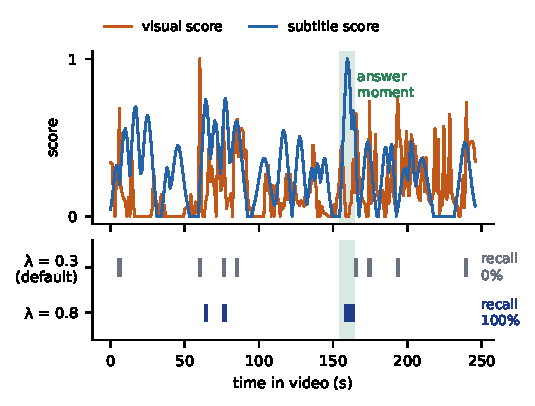
\includegraphics[width=\linewidth]{f01_teaser.pdf}\\
      {\scriptsize Real example: $\lam=0.3$ \bad{misses} the answer moment (green), $\lam=0.8$ \good{hits} it.}
    \end{column}
  \end{columns}
\end{frame}}

\newcommand{\titleframe}{%
{\setbeamertemplate{footline}{}\setbeamertemplate{frametitle}{}
\begin{frame}[t]\titlepage\end{frame}}}

\newcommand{\thankframe}{%
{\setbeamertemplate{footline}{}\setbeamertemplate{frametitle}{}
\begin{frame}[t]\mbzuaiThankYou\end{frame}}}
.
\usepackage{amsmath,amssymb}
\usepackage{booktabs}
\usepackage{xcolor}
\usetheme{MBZUAI}
\graphicspath{{assets/}{../figs/}}
\setbeamertemplate{navigation symbols}{}

\newcommand{\lam}{\lambda}
\newcommand{\strong}[1]{\textcolor{mbzuai-navy}{\textbf{#1}}}
\newcommand{\good}[1]{\textcolor{green!45!black}{\textbf{#1}}}
\newcommand{\bad}[1]{\textcolor{red!65!black}{\textbf{#1}}}

% ── Team and roles: edit here, all three decks update ─────────────────────
\newcommand{\roleJH}{Problem and setup; score cache and data pipeline; Q1 analysis; overall study (Q1--Q4)}
\newcommand{\roleLJ}{Continual learning experiments and analysis (Q2--Q3)}
\newcommand{\roleMA}{Downstream question-answering evaluation (Q4)}

\title[Fusion Weight for Keyframe Search]{Should the Fusion Weight Change with the Question?}
\institute[MBZUAI]{CV805 Course Project \\ Mohamed bin Zayed University of Artificial Intelligence}
\date{\today}
\titlelogos{assets/logo_dark.pdf}
\footleft{Should the Fusion Weight Change with the Question?}
\footright{\insertframenumber{} / \inserttotalframenumber}

% Team slide; #1 = JH, LJ or MA, the presenter's row is highlighted.
\usepackage{etoolbox}
\newcommand{\teamrow}[4]{% #1 key, #2 presenter key, #3 name, #4 role
  \ifstrequal{#1}{#2}%
    {\textbf{\textcolor{mbzuai-navy}{#3}} & \textbf{\textcolor{mbzuai-navy}{#4}} & \textcolor{mbzuai-dark-sand}{\textbf{this talk}}}%
    {\textcolor{mbzuai-subtle}{#3} & \textcolor{mbzuai-subtle}{#4} & }}
\newcommand{\teamframe}[1]{%
\begin{frame}{Team and my part}
  \centering
  \renewcommand{\arraystretch}{1.6}
  \begin{tabular}{p{0.27\textwidth}p{0.52\textwidth}p{0.11\textwidth}}
    \toprule
    Member & Main contribution & \\
    \midrule
    \teamrow{JH}{#1}{Jianxiang He}{\roleJH} \\
    \teamrow{LJ}{#1}{Longtao Jiang}{\roleLJ} \\
    \teamrow{MA}{#1}{Makhmud Assentay}{\roleMA} \\
    \bottomrule
  \end{tabular}
\end{frame}}

% Context frame used by every talk: VSI, the weight, and the example.
\newcommand{\contextframe}{%
\begin{frame}{Background: two clues, one weight}
  \begin{columns}[c,onlytextwidth]
    \begin{column}{0.47\textwidth}
      \small
      A VLM can only look at \strong{about 8 frames} of a long video, so we must pick them well.\\[2mm]
      VSI scores every second with two clues:
      \begin{itemize}
        \item \strong{Visual}: do the question's objects appear?
        \item \strong{Subtitle}: does the subtitle match the question?
      \end{itemize}
      \[ S(t) = (1-\lam)\,\text{visual}(t) + \lam\,\text{subtitle}(t) \]
      and keeps the top 8 seconds. VSI uses \strong{$\lam=0.3$ for every question}.
    \end{column}
    \begin{column}{0.5\textwidth}
      \centering
      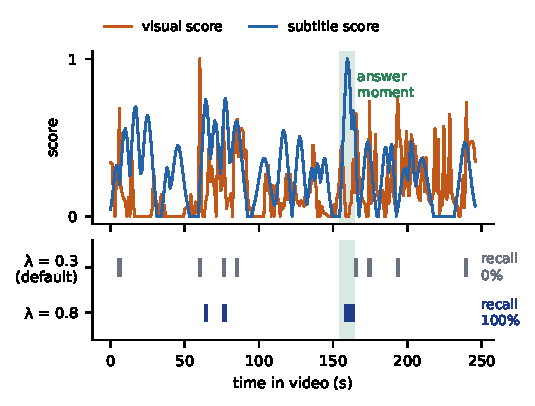
\includegraphics[width=\linewidth]{f01_teaser.pdf}\\
      {\scriptsize Real example: $\lam=0.3$ \bad{misses} the answer moment (green), $\lam=0.8$ \good{hits} it.}
    \end{column}
  \end{columns}
\end{frame}}

\newcommand{\titleframe}{%
{\setbeamertemplate{footline}{}\setbeamertemplate{frametitle}{}
\begin{frame}[t]\titlepage\end{frame}}}

\newcommand{\thankframe}{%
{\setbeamertemplate{footline}{}\setbeamertemplate{frametitle}{}
\begin{frame}[t]\mbzuaiThankYou\end{frame}}}
.
\usepackage{amsmath,amssymb}
\usepackage{booktabs}
\usepackage{xcolor}
\usetheme{MBZUAI}
\graphicspath{{assets/}{../figs/}}
\setbeamertemplate{navigation symbols}{}

\newcommand{\lam}{\lambda}
\newcommand{\strong}[1]{\textcolor{mbzuai-navy}{\textbf{#1}}}
\newcommand{\good}[1]{\textcolor{green!45!black}{\textbf{#1}}}
\newcommand{\bad}[1]{\textcolor{red!65!black}{\textbf{#1}}}

% ── Team and roles: edit here, all three decks update ─────────────────────
\newcommand{\roleJH}{Problem and setup; score cache and data pipeline; Q1 analysis; overall study (Q1--Q4)}
\newcommand{\roleLJ}{Continual learning experiments and analysis (Q2--Q3)}
\newcommand{\roleMA}{Downstream question-answering evaluation (Q4)}

\title[Fusion Weight for Keyframe Search]{Should the Fusion Weight Change with the Question?}
\institute[MBZUAI]{CV805 Course Project \\ Mohamed bin Zayed University of Artificial Intelligence}
\date{\today}
\titlelogos{assets/logo_dark.pdf}
\footleft{Should the Fusion Weight Change with the Question?}
\footright{\insertframenumber{} / \inserttotalframenumber}

% Team slide; #1 = JH, LJ or MA, the presenter's row is highlighted.
\usepackage{etoolbox}
\newcommand{\teamrow}[4]{% #1 key, #2 presenter key, #3 name, #4 role
  \ifstrequal{#1}{#2}%
    {\textbf{\textcolor{mbzuai-navy}{#3}} & \textbf{\textcolor{mbzuai-navy}{#4}} & \textcolor{mbzuai-dark-sand}{\textbf{this talk}}}%
    {\textcolor{mbzuai-subtle}{#3} & \textcolor{mbzuai-subtle}{#4} & }}
\newcommand{\teamframe}[1]{%
\begin{frame}{Team and my part}
  \centering
  \renewcommand{\arraystretch}{1.6}
  \begin{tabular}{p{0.27\textwidth}p{0.52\textwidth}p{0.11\textwidth}}
    \toprule
    Member & Main contribution & \\
    \midrule
    \teamrow{JH}{#1}{Jianxiang He}{\roleJH} \\
    \teamrow{LJ}{#1}{Longtao Jiang}{\roleLJ} \\
    \teamrow{MA}{#1}{Makhmud Assentay}{\roleMA} \\
    \bottomrule
  \end{tabular}
\end{frame}}

% Context frame used by every talk: VSI, the weight, and the example.
\newcommand{\contextframe}{%
\begin{frame}{Background: two clues, one weight}
  \begin{columns}[c,onlytextwidth]
    \begin{column}{0.47\textwidth}
      \small
      A VLM can only look at \strong{about 8 frames} of a long video, so we must pick them well.\\[2mm]
      VSI scores every second with two clues:
      \begin{itemize}
        \item \strong{Visual}: do the question's objects appear?
        \item \strong{Subtitle}: does the subtitle match the question?
      \end{itemize}
      \[ S(t) = (1-\lam)\,\text{visual}(t) + \lam\,\text{subtitle}(t) \]
      and keeps the top 8 seconds. VSI uses \strong{$\lam=0.3$ for every question}.
    \end{column}
    \begin{column}{0.5\textwidth}
      \centering
      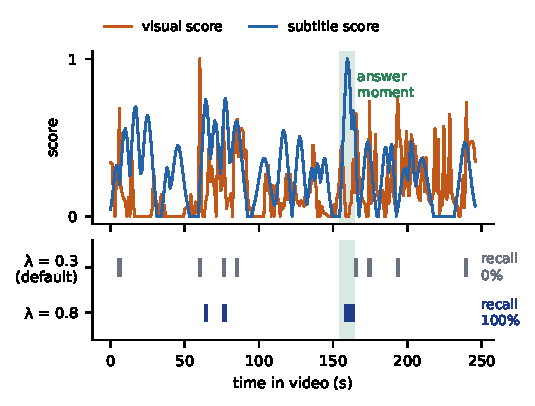
\includegraphics[width=\linewidth]{f01_teaser.pdf}\\
      {\scriptsize Real example: $\lam=0.3$ \bad{misses} the answer moment (green), $\lam=0.8$ \good{hits} it.}
    \end{column}
  \end{columns}
\end{frame}}

\newcommand{\titleframe}{%
{\setbeamertemplate{footline}{}\setbeamertemplate{frametitle}{}
\begin{frame}[t]\titlepage\end{frame}}}

\newcommand{\thankframe}{%
{\setbeamertemplate{footline}{}\setbeamertemplate{frametitle}{}
\begin{frame}[t]\mbzuaiThankYou\end{frame}}}
.
\usepackage{amsmath,amssymb}
\usepackage{booktabs}
\usepackage{xcolor}
\usetheme{MBZUAI}
\graphicspath{{assets/}{../figs/}}
\setbeamertemplate{navigation symbols}{}

\newcommand{\lam}{\lambda}
\newcommand{\strong}[1]{\textcolor{mbzuai-navy}{\textbf{#1}}}
\newcommand{\good}[1]{\textcolor{green!45!black}{\textbf{#1}}}
\newcommand{\bad}[1]{\textcolor{red!65!black}{\textbf{#1}}}

% ── Team and roles: edit here, all three decks update ─────────────────────
\newcommand{\roleJH}{Problem and setup; score cache and data pipeline; Q1 analysis; overall study (Q1--Q4)}
\newcommand{\roleLJ}{Continual learning experiments and analysis (Q2--Q3)}
\newcommand{\roleMA}{Downstream question-answering evaluation (Q4)}

\title[Fusion Weight for Keyframe Search]{Should the Fusion Weight Change with the Question?}
\institute[MBZUAI]{CV805 Course Project \\ Mohamed bin Zayed University of Artificial Intelligence}
\date{\today}
\titlelogos{assets/logo_dark.pdf}
\footleft{Should the Fusion Weight Change with the Question?}
\footright{\insertframenumber{} / \inserttotalframenumber}

% Team slide; #1 = JH, LJ or MA, the presenter's row is highlighted.
\usepackage{etoolbox}
\newcommand{\teamrow}[4]{% #1 key, #2 presenter key, #3 name, #4 role
  \ifstrequal{#1}{#2}%
    {\textbf{\textcolor{mbzuai-navy}{#3}} & \textbf{\textcolor{mbzuai-navy}{#4}} & \textcolor{mbzuai-dark-sand}{\textbf{this talk}}}%
    {\textcolor{mbzuai-subtle}{#3} & \textcolor{mbzuai-subtle}{#4} & }}
\newcommand{\teamframe}[1]{%
\begin{frame}{Team and my part}
  \centering
  \renewcommand{\arraystretch}{1.6}
  \begin{tabular}{p{0.27\textwidth}p{0.52\textwidth}p{0.11\textwidth}}
    \toprule
    Member & Main contribution & \\
    \midrule
    \teamrow{JH}{#1}{Jianxiang He}{\roleJH} \\
    \teamrow{LJ}{#1}{Longtao Jiang}{\roleLJ} \\
    \teamrow{MA}{#1}{Makhmud Assentay}{\roleMA} \\
    \bottomrule
  \end{tabular}
\end{frame}}

% Context frame used by every talk: VSI, the weight, and the example.
\newcommand{\contextframe}{%
\begin{frame}{Background: two clues, one weight}
  \begin{columns}[c,onlytextwidth]
    \begin{column}{0.47\textwidth}
      \small
      A VLM can only look at \strong{about 8 frames} of a long video, so we must pick them well.\\[2mm]
      VSI scores every second with two clues:
      \begin{itemize}
        \item \strong{Visual}: do the question's objects appear?
        \item \strong{Subtitle}: does the subtitle match the question?
      \end{itemize}
      \[ S(t) = (1-\lam)\,\text{visual}(t) + \lam\,\text{subtitle}(t) \]
      and keeps the top 8 seconds. VSI uses \strong{$\lam=0.3$ for every question}.
    \end{column}
    \begin{column}{0.5\textwidth}
      \centering
      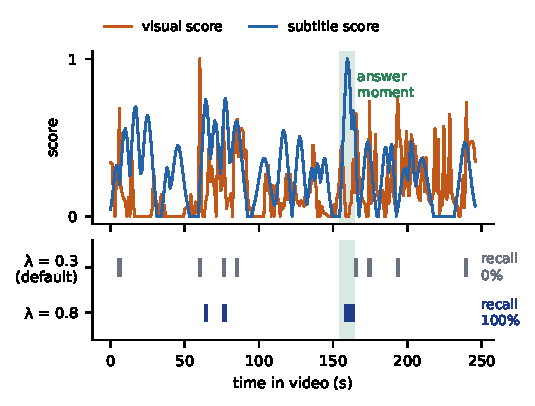
\includegraphics[width=\linewidth]{f01_teaser.pdf}\\
      {\scriptsize Real example: $\lam=0.3$ \bad{misses} the answer moment (green), $\lam=0.8$ \good{hits} it.}
    \end{column}
  \end{columns}
\end{frame}}

\newcommand{\titleframe}{%
{\setbeamertemplate{footline}{}\setbeamertemplate{frametitle}{}
\begin{frame}[t]\titlepage\end{frame}}}

\newcommand{\thankframe}{%
{\setbeamertemplate{footline}{}\setbeamertemplate{frametitle}{}
\begin{frame}[t]\mbzuaiThankYou\end{frame}}}
